\documentclass{article}

\usepackage{graphicx}
\usepackage{tikz}
\usepackage{tikzsymbols}
\usetikzlibrary{calc,patterns,shapes.geometric}
\pagestyle{empty}
\usepackage[margin=0pt]{geometry}
\geometry{papersize={14in,12in}}

\def\centerarc[#1](#2)(#3:#4:#5){\draw[#1] ($(#2)+({#5*cos(#3)},{#5*sin(#3)})$) arc (#3:#4:#5);}

\begin{document}
	\begin{figure}
		\centering
		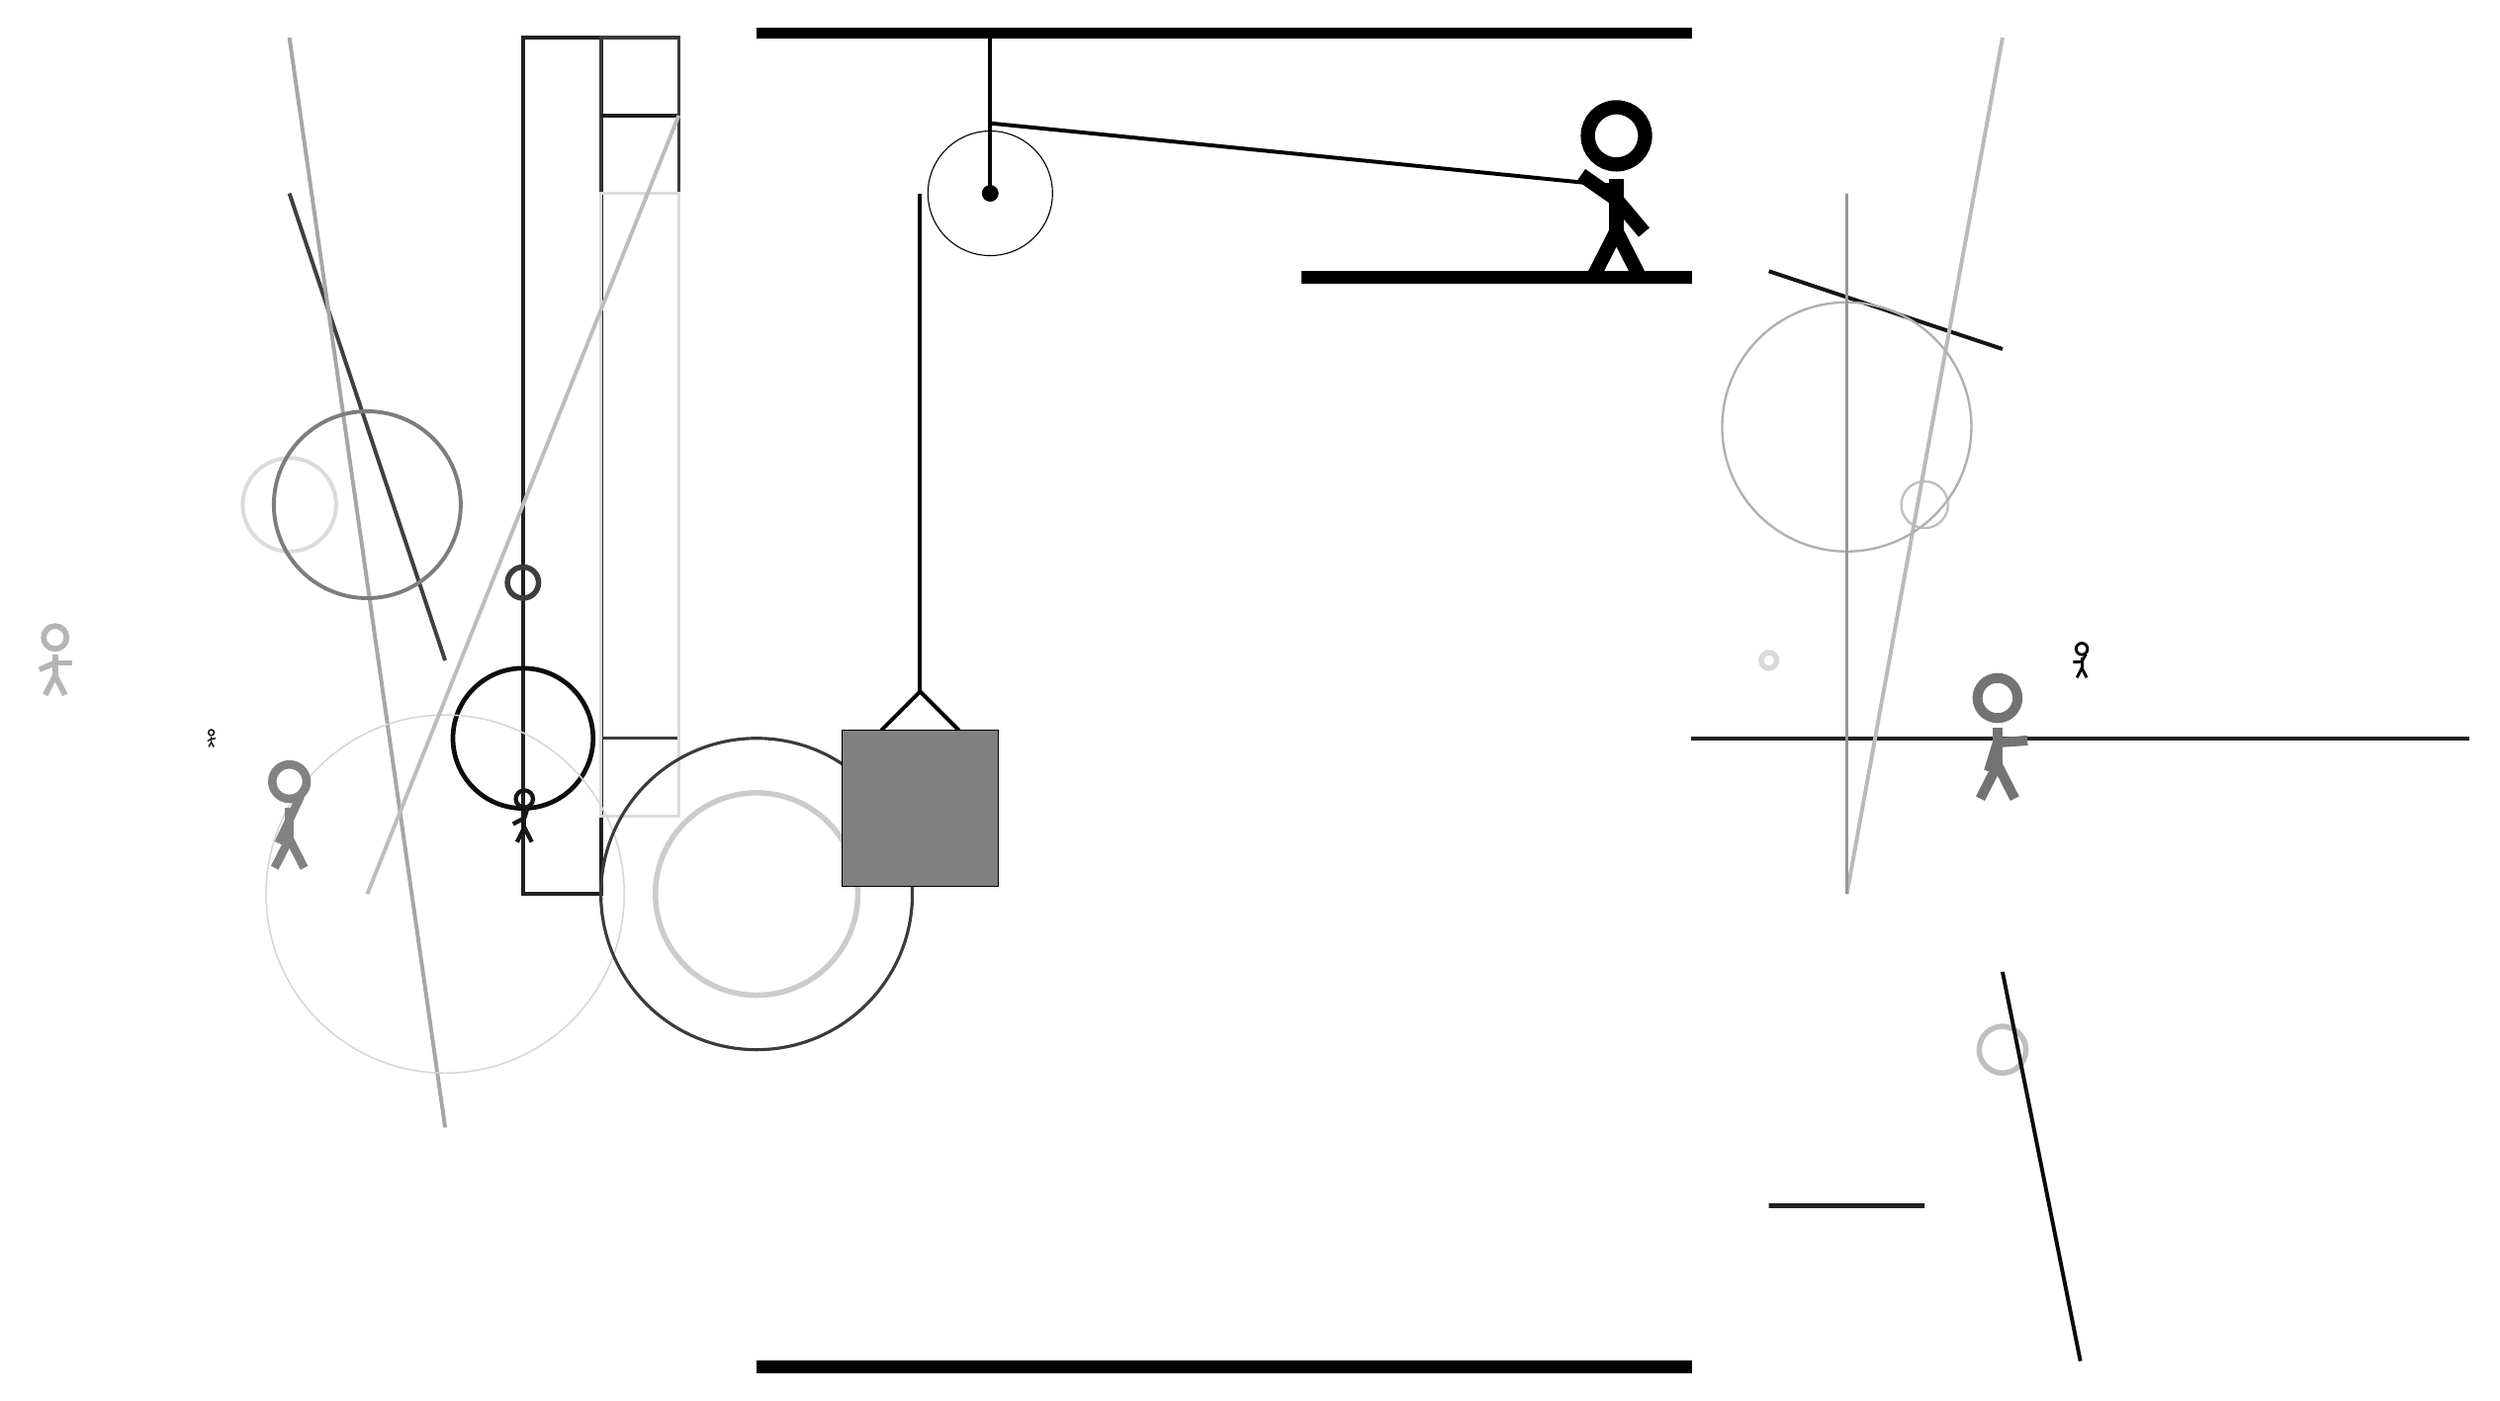
\begin{tikzpicture}
			%%%%% START %%%%%
			
			\draw[fill=black] (-2, 14) rectangle (10, 14.125);
			
			\draw (1, 12) circle (0.8);
			\draw[fill=black] (1, 12) circle (0.1);
			\draw[line width=0.5mm] (1, 14) -- (1, 12);
			
			\draw [line width=0.3mm, color=black!25](13, 8) circle (0.3);
			
			\draw [line width=0.5mm, color=black!14](-8, 8) circle (0.6);
			\draw[line width=0.5mm, color=black!75](-6, 6) -- (-8, 12);
			\draw[line width=0.5mm, color=black!92](14, 10) -- (11, 11);
			
			\draw [line width=0.7mm, color=black!15](11, 6) circle (0.1);
			\draw[line width=0.5mm, color=black!35](-6, 0) -- (-8, 14);
			\draw [line width=0.7mm, color=black!25](14, 1) circle (0.3);
			\draw[line width=0.5mm, color=black!86](10, 5) -- (20, 5);
			\draw[line width=0.5mm, color=black!87] (-4, 14) rectangle (-5, 3);
			\draw[line width=0.5mm, color=black!27](12, 3) -- (14, 14);
			\node[line width=0.5mm, color=black!97] at (-9, 5) {\Strichmaxerl[1][29][6]};
			\draw [line width=0.7mm, color=black!76](-5, 7) circle (0.2);
			\draw[line width=0.4mm, color=black!77] (-4, 5) rectangle (-3, 14);
			
			\draw [line width=0.3mm, color=black!31](12, 9) circle (1.6);
			\node[line width=0.2mm, color=black!29] at (-11, 6) {\Strichmaxerl[4][23][0]};
			\draw [line width=0.5mm, color=black!51](-7, 8) circle (1.2);
			
			\draw [line width=0.6mm, color=black!95](-5, 5) circle (0.9);
			
			\draw[line width=0.6mm, color=black!87] (11, -1) rectangle (13, -1);
			\draw[line width=0.4mm, color=black!14] (-4, 12) rectangle (-3, 4);
			
			\node[line width=0.6mm, color=black!55] at (14, 5) {\Strichmaxerl[7][73][4]};
			\draw [line width=0.2mm, color=black!16](-6, 3) circle (2.3);
			
			\draw [line width=0.4mm, color=black!77](-2, 3) circle (2.0);
			\draw[line width=0.5mm, color=black!41] (12, 12) rectangle (12, 3);
			\draw[line width=0.5mm, color=black!88] (-4, 13) rectangle (-3, 13);
			\node[line width=0.6mm, color=black!91] at (-5, 4) {\Strichmaxerl[3][28][73]};
			
			\draw[line width=0.5mm, color=black!26](-3, 13) -- (-7, 3);
			\node[line width=0.2mm, color=black!100] at (15, 6) {\Strichmaxerl[2][2][61]};
			\draw[line width=0.5mm, color=black!96](15, -3) -- (14, 2);
			\draw [line width=0.7mm, color=black!20](-2, 3) circle (1.3);
			
			\node[line width=0.2mm, color=black!49] at (-8, 4) {\Strichmaxerl[6][65][65]};
			
			\draw[line width=0.5mm](-0.4, 5.1) --  (0.1, 5.6) -- (0.6, 5.1);
			\draw[fill=black!50] (-0.9, 5.1) rectangle (1.1, 3.1);
			
			\draw[line width=0.5mm](0.1, 12) -- (0.1, 5.6);
			\centerarc[line width=0.5mm](1, 12)(90:180:0.9)
			\draw[line width=0.5mm](1, 12.9) -- (9, 12.1);
			
			\node at (9, 12) {\Strichmaxerl[10][-35][-50]};
			\draw[fill=black] (5, 11) rectangle (10, 10.85);
			
			\draw[fill=black] (-2, -3) rectangle (10, -3.15);
			
			%%%%% END %%%%%
		\end{tikzpicture}
	\end{figure}	
\end{document}